\documentclass{standalone}
\usepackage{tikz}
\begin{document}
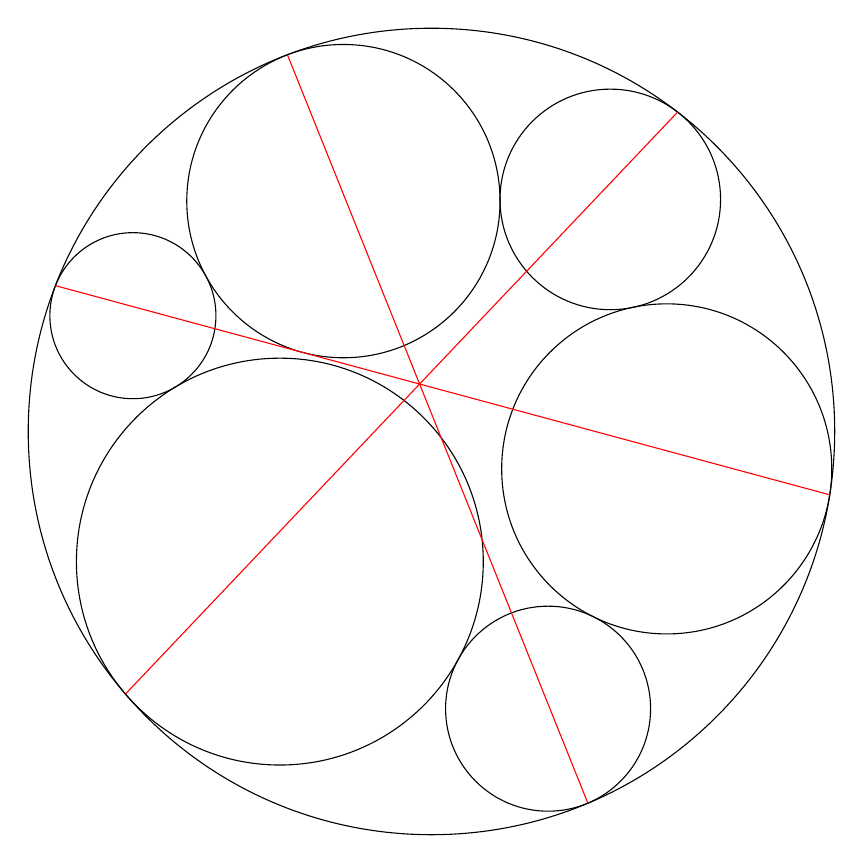
\begin{tikzpicture}[x=1pt,y=1pt]
\draw (150.00,-150.00) circle (145.71);
\draw (42.11,-108.16) circle (30.00);
\draw (95.21,-197.02) circle (73.51);
\draw (192.14,-250.17) circle (37.04);
\draw (235.01,-163.52) circle (59.64);
\draw (214.62,-66.15) circle (39.85);
\draw (118.18,-66.76) circle (56.60);
\draw[red] (14.14,-97.32) -- (293.91,-172.89);
\draw[red] (39.42,-244.89) -- (238.95,-34.59);
\draw[red] (206.51,-284.31) -- (97.96,-13.89);
\end{tikzpicture}
\end{document}
